\section{实验评估}\label{sec:eval}
实验围绕四个问题展开：共同来源推理是否带来实质分析精度变化（RQ1）；完整支持及大规模选定查询是否与独立语义一致（RQ2）；完整诊断任务能增长到何种规模、哪些因素决定成本（RQ3）；改变同步拓扑后，同一定理是否仍能解释候选结构（RQ4）。所有表格来自冻结结果，失败状态与成功记录一并保留。

\subsection{设置、基线与计时口径}
主要输入是第~\ref{sec:separation}节的 $P(n,2)$ 和 $\pv(n,2)$。前者反复写常量 1，后者记录轮次版本。两者有完全相同的同步拓扑和程序序，但版本值排除了跨轮数据 RF；两者的规模结果必须分开解释。它们是可执行研究内核，已有 C11／pthread 和 litmus 导出，未声称从工业库抽取或验证了任意自旋重试。

正式计时在同一 Linux x86\_64 主机上进行，Python 3.10.12，绑定 CPU 0，串行运行。每个配置成功重复三次，报告中位数；第一次资源失败后停止该配置。内存上限 4 GiB，构造时间上限 90 秒，总 wall 上限 240 秒；图预算为 $10^6$ 累计状态、$3\times10^6$ 边。64 轮为单独压力点，仅运行一次，状态／边预算提高为 $2\times10^6/6\times10^6$，其余限制相同。时间包括构造及完整客户端任务，不以单次传播微基准代替总成本。

端口方法包括原子 RF、二元 RF、关闭共同前序规则和关闭原生扩展的消融。SAT 对照使用独立稠密 RA 编码与 Minisat：SAT-full 每次求全部原始支持；SAT-demand 在冲突提取时仅求一致性，修复时只求相关字段全部值，完整快照仍求全部支持。BDD 对照使用 CUDD 后端和 coherence 优先的关系编码，执行同一诊断合同。这些是明示实现的比较，不代表 Dat3M、GenMC 或所有 SAT／BDD 技术的最佳性能。新增 CaDiCaL incidence 编码单独用于正确性核对，不混入这组历史计时。

\subsection{RQ1：与原生关系分析的实质对照}\label{sec:native}
最接近的分析框架是 Haas 等的 may/must 过滤方法~\cite{haas2023}。我们实际调用 Dat3M 4.5.0-alpha 的原生 \texttt{NativeRelationAnalysis}，启用扩展关系分析；提交为 \texttt{b81ec6c55503}（完整摘要见制品）。这是 2026 年实现审计，不是重跑 2023 年论文制品的性能结果。适配器不修改 Dat3M 源码、不重写原生传播器、不调用 SMT 搜索。

两方输入使用相同固定读值 RF 域和相同 RA CAT 公理，并逐事件核对映射；否则，默认分析未获得固定读值会造成不公平的输入差异。四种配置依次提供：仅值域、$K_0$ 事实、$K_0+R_\forall$、以及再补入 HB／CO 闭包和必要删域的完整外部过滤。表~\ref{tab:native} 报告恒定载荷的结果。

\begin{table}[tb]
\caption{原生分析精度审计。关键 HB 是“上轮首次发布到本轮等待”；末列指完整外部过滤与 $\ka$ 的 $H,L,D$ 集合相等。}\label{tab:native}
\centering\small
\begin{tabular}{rrrrcl}\toprule
$n$ & 仅值域 RF & $K_0$ RF & $\ka$ RF & $K_0$ 缺失关键 HB & 完整集合相等\\\midrule
\tableinput tables/native_rows.tex 
\bottomrule\end{tabular}
\end{table}

$K_0$ 输入已提供来源块，但原生输出仍缺少全部关键共同 HB。单独加入 $R_\forall$ 恢复这些边；再执行固定片段的必要闭包与删域，则在 $n=1,2,3,4,8,16$ 全部六项中，与 $\ka$ 的 $H,L,D$ \emph{完整集合}一致。由此得到两个结论：共同来源事实对候选缩减有实质作用；这些事实可接入已有框架，不能把默认实现的缺失解释成框架表达能力不足。定理~\ref{thm:main} 的新义务仍是块锁定、网络传播、覆盖边局部性及参数界。Java 启动成本不用于分析速度比较。

\subsection{RQ2：语义正确性与 32 轮独立核对}
验证分为数学论证、独立实现交叉和完整见证复查。小规模测试枚举原始部分赋值，与不调用识别器的稠密 RA 定义核对；来源、CO 常量、冲突、负 RF 假设与撤销均在原始合同内。正式任务中所有已完成方法和重复运行的完整诊断结果一致；版本载荷至 16 轮有独立稠密 SAT 完整支持对照，BDD 完整对照至 8 轮。表~\ref{tab:validation} 区分各种证据的覆盖范围。

\begin{table}[tb]
\caption{正确性证据及其范围。“选定”不表示穷尽所有假设或所有目标。}\label{tab:validation}
\small\begin{tabularx}{\textwidth}{p{2.5cm}Y Y}\toprule
证据 & 已完成核查 & 能支持的结论\\\midrule
小固定输入 & 新 oracle 的 20 个随机输入全部原始部分赋值，与穷举 RA 一致 & 独立编码的有限语义交叉\\
原有完整任务 & 所有已完成方法与重复结果相同；版本 16 轮 SAT、8 轮 BDD 对照 & 所测诊断查询的全支持一致\\
32 轮选定核对 & 53 场景，826 个目标文字，879 次 SAT 调用；81 个完整见证 & 所选一致性与文字支持一致\\
有向环 & 五个已完成配置逐查询全部原始支持一致；最小环另验纯 UP & 不同拓扑下的实现正确性证据\\
结构核查 & 12 个实例、3,360 个整数窗口及两个前提反例 & 检查具体证书与边界实现\\
干净环境复现 & 50 项测试通过，1 项 CUDD 测试跳过；全部新增实验重跑 & 安装、源码构建与结果可复现\\\bottomrule
\end{tabularx}
\end{table}

32 轮输入含 388 个事件、10,528 个原始位。我们选取阶段 $2,8,16,24,32$，覆盖两线程早／晚来源、倒置 CO、撤销，以及额外负 RF 和否定初始化来源假设，共 53 个场景。新 oracle 使用 CaDiCaL 1.9.5，以实际基本边的右扩展约束表达 HB，独立编码 RF、CO 和 coherence；不调用 $\ka$、端口、布局或 $D/H/L$ 证书。其等价性证明见附录~\ref{app:oracle}。

53 个一致性结果与 826 个正／负目标支持全部相同；41 个场景的完整图答案摘要与旧冻结记录相同，其余为新增查询。可行支持引用 81 个不同完整 RF／CO 赋值，逐一重算 HB／ECO 闭包验证。目标包括条件 CO、同轮两位数据写者、早／晚同步来源、远期排除来源及原始常量。UNSAT 由独立求解器给出，本轮没有生成 DRAT 证明。因此，这些实验增强大规模可信度，但不代替任意 $\alpha$ 下的数学保证。

新编码含 5,131,294 条子句、160,684 个 CNF 变量；原始构造约 13.41 秒，核对阶段约 25.64 秒，后者还包括图查询、见证解码、稠密验证和保存。整个进程峰值 RSS 为 571,800 KiB，允许 8 GiB 内存。它完成的任务与正式完整客户端不同，预算也不同，不能与表~\ref{tab:times} 计算速度比。尤其，旧稠密编码的 32 轮失败不能概括为“SAT 在 32 轮不可行”。

\subsection{RQ3：完整任务增长及机制拆分}
表~\ref{tab:times} 给出版本载荷的完整诊断时间。32 轮原子端口方法完成 249 份报告、621 次支持接口调用，总时间中位数为 16.070 秒。64 轮单次压力点完成 505 份报告和 1,261 次调用，总时间 77.175 秒，峰值 RSS 约 495 MiB；它没有此次独立大规模核对，也不作为重复性能结论。

\begin{table}[tb]
\caption{版本载荷 $\pv(n,2)$ 的完整诊断时间（秒，含构造）。除 $64^*$ 为单次外，成功项为三次中位数。UNK 表示资源超限，ERR 为内存错误报告异常，-- 为未测。}\label{tab:times}
\centering\footnotesize\setlength{\tabcolsep}{3.5pt}
\begin{tabular}{rrr rrrrr}\toprule
$n$ & 事件 & $|X|$ & 端口原子 & 端口二元 & SAT-full & SAT-demand & BDD\\\midrule
\tableinput tables/timing_rows.tex 
\bottomrule\end{tabular}
\end{table}

四轮时 SAT-demand 用时 0.316 秒，快于原子端口的 0.408 秒；八、十六轮时，本组实现中端口完整任务更快。32 轮二元组达到状态预算，稠密 SAT-full 达到 4 GiB 限制，SAT-demand 在内存不足后的错误报告过程又触发异常；BDD 在十六、三十二轮达到 240 秒总时限。所有失败均保留原始状态，不视为 UNSAT，也不以时限替代真实完成时间。图~\ref{fig:times} 只连接已完成点。

\begin{figure}[tb]
\centering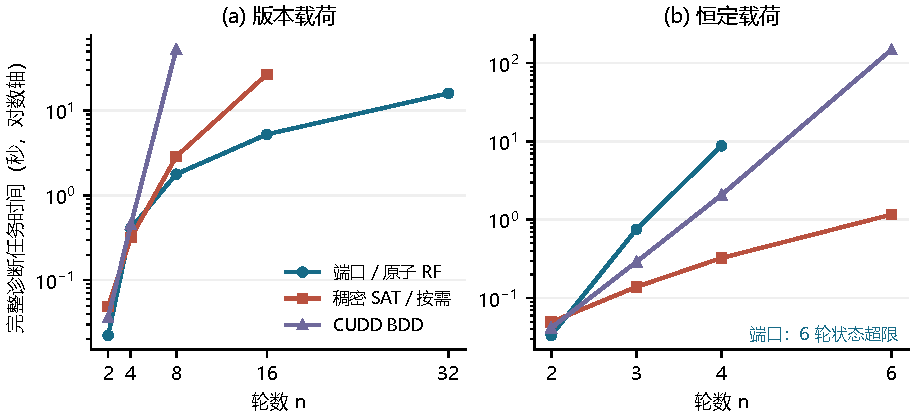
\includegraphics[width=\textwidth]{task_times.pdf}
\caption{同一诊断合同下的总时间。左为版本载荷，右为恒定载荷；缺少数据点表示未完成或未测，具体状态见表。SAT 曲线仅代表该稠密编码的按需实现。}\label{fig:times}
\end{figure}

\begin{table}[tb]
\caption{版本载荷的图规模与任务规模。累计构造状态包含后处理前的状态；后缀商不会消除已发生的构造成本。}\label{tab:size}
\centering\small\setlength{\tabcolsep}{4pt}
\begin{tabular}{r rrr rrr}\toprule
$n$ & 累计状态 & 商后状态 & 最大单层 & 构造秒 & 报告 & 调用\\\midrule
\tableinput tables/size_rows.tex 
\bottomrule\end{tabular}
\end{table}

图~\ref{fig:scaling} 与表~\ref{tab:size} 区分整体规模和每层状态数。版本载荷已测 $n\ge8$ 的最大单层状态数为 1,230；累计状态从八轮 128,666 增长到三十二轮 709,082，商后图从 4,842 增长到 22,554。理论仅保证固定结构参数下的统一上界，不能由这些点推断精确线性运行时间。原始 CO 输出仍随 $n$ 二次增长，客户端解码与报告构造也不可忽略。64 轮中，核心支持查询累计约 15.55 秒，而完整客户端阶段约 42.19 秒。

\begin{figure}[tb]
\centering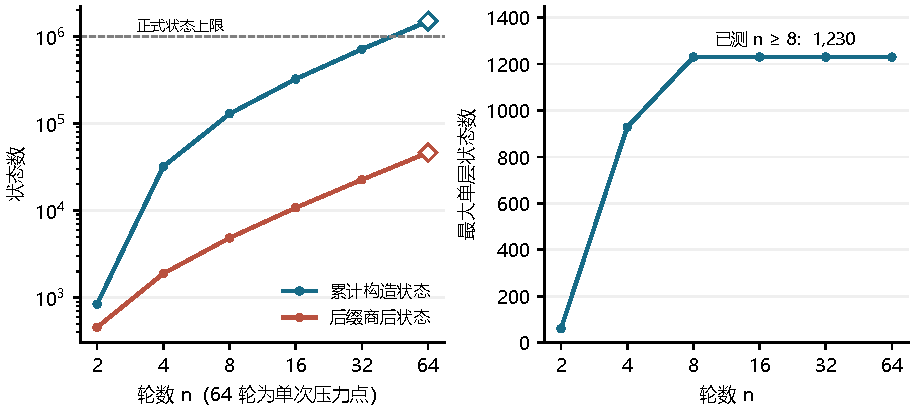
\includegraphics[width=\textwidth]{graph_scaling.pdf}
\caption{版本载荷的构造规模。空心菱形标记提高状态预算后的 64 轮单次点；1,230 是实测单层值，不是一般定理常数。}\label{fig:scaling}
\end{figure}

机制消融给出更明确的因果解释。四轮关闭共同前序，累计状态由 31,930 增为 150,847，完整时间从 0.408 秒增为 2.374 秒；八轮无共同前序达到状态上限。原子 RF 比二元 RF 减少无效局部组合，八轮累计状态从 185,337 减至 128,666。关闭 C++ 后，四／八轮构造从 0.384／1.639 秒变为 2.852／12.615 秒，状态数完全相同；八轮纯 Python 完整任务为 12.758 秒，慢于 SAT-demand。因而实际时间收益同时依赖表示和实现，不能全部归于定理。

恒定载荷给出必要的负面对照（表~\ref{tab:constant}）。四轮原子端口已需 8.783 秒，六轮超过一百万状态；SAT-demand 六轮仍在 1.167 秒完成。恒定载荷允许大量跨轮同值来源，虽仍满足局部化定理，实际状态常数却显著增大。版本载荷的可扩展性部分来自额外观测信息，这不是在相同输入上凭算法消除了困难。

\begin{table}[tb]
\caption{恒定载荷 $P(n,2)$ 的完整任务时间（秒，三次中位数）。}\label{tab:constant}
\centering\begin{tabular}{rrrr}\toprule
$n$ & 端口原子 & SAT-demand & BDD\\\midrule
\tableinput tables/constant_rows.tex 
\bottomrule\end{tabular}
\end{table}

\subsection{RQ4：不同同步拓扑}
为了使结构变化超出双线程加轮数，我们构造有向环上的邻居状态交换。对 $p\ge3$，线程 $t$ 在阶段 $i$ 依次执行
\begin{align*}
 W(x_t,i);\ W(f_t,b_i)_0;\ W(x_{t+1},i);\ W(f_t,b_i)_1;\qquad\\
 R(f_{t-1},b_{i-1});\ R(x_t,i),
\end{align*}
下标按 $p$ 取模。每数据地址有两位写者，每标志只有一位写者。另一个变体让各线程／阶段交替使用两次或三次发布，检查定理不依赖固定块长。这是有实际状态交换含义的有限内核，未冒称某工业协议的完整实现。

三线程时 $d=2,b=18,a=6,G=1$，因此 $h=5,\delta=11,k=222,k_A=420$。因果证据可能经过中间线程，已不同于双线程直接互相同步。图~\ref{fig:ring} 展示结构扫描：十六轮时未决 CO 从 $K_0$ 的 768 对减到 $\ka$ 的 261 对，仍有 45 个多来源等待；八／十六轮实际事件袋大小为 33。故局部化并未把原始不确定性全部固定。

\begin{figure}[tb]
\centering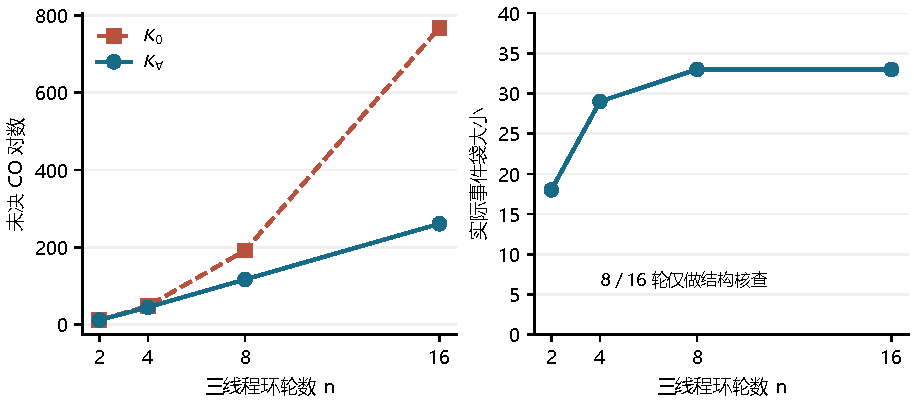
\includegraphics[width=\textwidth]{ring_structure.pdf}
\caption{三线程有向环的结构核查。较大轮数只核查候选与布局，并不表示完成完整支持编译。}\label{fig:ring}
\end{figure}

\begin{table}[tb]
\caption{不同拓扑的单次正确性实验。三线程四轮在累计 1,000,001 状态时停止，未产生一致性答案；其他配置对所有原始位核对完整支持。}\label{tab:ring}
\centering\footnotesize\setlength{\tabcolsep}{3pt}
\begin{tabular}{lrrrrrl}\toprule
配置 & 事件 & $|X|$ & 累计状态 & 商后状态 & 场景 & 状态\\\midrule
\tableinput tables/ring_rows.tex 
\bottomrule\end{tabular}
\end{table}

表~\ref{tab:ring} 中五个完成配置的全原始支持均与独立 CaDiCaL 一致；三线程两轮另验支持 CNF 的纯 UP。所有可行查询均保存完整 RF／CO 见证并重算 RA。最小环的独立 SC 全序编码为 UNSAT，与前述一般论证一致。三线程三轮关闭共同前序后状态数完全相同，此规模上没有额外缩图收益；四轮则在标准预算下失败。这说明同一定理仍解释不同拓扑的候选局部性，但较大的接口足以使实际编译变贵。

\subsection{复现与有效性边界}
制品提供生成器、算法、独立 oracle、查询输入、完整见证、失败记录和逐文件 SHA-256 清单。我们在全新目录与全新虚拟环境中，从源码编译原生扩展并完整复跑新增核查：51 项测试中 50 项通过，1 项因未安装 CUDD 跳过；原完整依赖环境的 51 项全部通过。53 场景／826 支持核对以及全部环配置的状态与图规模均复现。干净环境全流程约 115 秒，此时间是复现回执而非基准性能。

实验不提供工业代表性或普遍速度优势。三次重复仅降低计时偶然性，不能消除构造族选择偏差；图中的中位数不是置信区间。64 轮仅为一次压力点；32 轮独立核对只覆盖选定目标；小实例穷举和测试不等于机器认证的一般证明。强 SAT 编码已经改变 32 轮的可行性，因此论文的主要经验结论是“定理可落地、完整支持可消费、失败可解释”，而非“编译全面胜过 SAT”。
\FloatBarrier
